\documentclass[12pt]{scrartcl}

\usepackage[T1]{fontenc}
\usepackage[utf8]{inputenc}
\usepackage{amsmath}
\usepackage{amsfonts}
\usepackage{amssymb}
\usepackage{amsbsy}
\usepackage{graphicx}
\usepackage{float}
\usepackage{array}
\usepackage{booktabs}
\usepackage{multirow}
\usepackage{bm}
\usepackage{verbatim}
\usepackage[english]{babel}
\usepackage{color}
\usepackage{url}
\usepackage{fancybox}
\usepackage[stable]{footmisc}
\usepackage[format=plain,labelfont=bf]{caption}
\usepackage{fancyhdr}
\usepackage{natbib}
\usepackage{calc}
\usepackage{textcomp}
\usepackage[pdftex,pdfborder={0 0 0}]{hyperref}
\usepackage{pdfpages}
\usepackage{tikz}
\usetikzlibrary{shapes,backgrounds,fit,shadows,arrows,positioning}
\usepackage{mathtools}
\usepackage{algorithm}
\usepackage{algorithmic}
\usepackage{placeins}
% Define the layers to draw the diagram
\pgfdeclarelayer{background}
\pgfdeclarelayer{foreground}
\pgfsetlayers{background,main,foreground}
\pagenumbering{gobble}

% Define block styles
\tikzstyle{process} = [draw, fill=blue!20, text centered, text width=13em, minimum width=8em, minimum height=3em, rounded corners, drop shadow,font=\bfseries]
\tikzstyle{inputdata} = [draw, fill=green!20, text centered, text width=4em, minimum width=3em, minimum height=3em, drop shadow,font=\bfseries]
\tikzstyle{tmpdata} = [draw, fill=orange!20, text centered, text width=4em, minimum width=3em, minimum height=3em, drop shadow,font=\bfseries]
\tikzstyle{outputdata} = [draw, fill=red!20, text centered, text width=4em, minimum width=3em, minimum height=3em, drop shadow,font=\bfseries]
\tikzstyle{indexdata} = [draw, text centered, text width=2.5em, minimum width=2em, minimum height=2em, rounded corners, font=\bfseries]
\tikzstyle{arrow} = [draw, ultra thick, color=black!50, -latex']
\tikzstyle{line} = [draw, ultra thick, color=black!50]
\tikzstyle{dash} = [dotted, draw, ultra thick, color=black!50, -latex']
\tikzstyle{layer} = [draw, fill=blue!20, text centered, text width=\linewidth, minimum width=8em, minimum height=3em, rounded corners, drop shadow,font=\bfseries]

% Define distances for bordering
\newcommand{\blockdist}{1.3}
\newcommand{\edgedist}{1.5}
\newcommand{\inputdata}[2]{node (i#1) [inputdata] {#2}}
\newcommand{\tmpdata}[2]{node (t#1) [tmpdata] {#2}}
\newcommand{\outputdata}[2]{node (o#1) [outputdata] {#2}}
\newcommand{\indexdata}[2]{node (d#1) [indexdata] {#2}}
\newcommand{\process}[2]{node (p#1) [process] {#2}}
\newcommand{\layer}[2]{node (l#1) [layer] {#2}}
\newcommand{\background}[7]{%
\begin{pgfonlayer}{background}
% Left-top corner of the background rectangle
\path (#1.west |- #2.north)+(-0.5,0.25) node (a1) {};
% Right-bottom corner of the background rectanle
\path (#3.east |- #4.south)+(+0.5,-0.25) node (a2) {};
% Draw the background
\path[fill=#6!20,rounded corners, draw=black!50, dashed] (a1) rectangle (a2);
\path (#3.east |- #2.north)+(0,0.25)--(#1.west |- #2.north) node[midway] (#5-n) {};
\path (#3.east |- #2.south)+(0,-0.35)--(#1.west |- #2.south) node[midway] (#5-s) {};
\path (#3.east |- #2.north)+(0.7,0)--(#3.east |- #4.south) node[midway] (#5-w) {};
% Write test
\node[below of=#4,node distance = 1.3cm, text centered, text width=12em, minimum width=8em, minimum height=3em,font=\bfseries] (tmp) {#7};
\end{pgfonlayer}}

\renewcommand*{\familydefault}{\sfdefault}

% Margins
\addtolength{\textheight}{1.0cm}
\addtolength{\oddsidemargin}{-0.5cm}
\addtolength{\evensidemargin}{-0.5cm}
\addtolength{\textwidth}{1.0cm}
\parindent=0em

% Appropriate font for \mathcal{}
\DeclareSymbolFont{cmmathcal}{OMS}{cmsy}{m}{n}
\DeclareSymbolFontAlphabet{\mathcal}{cmmathcal}

% Set subscript and superscripts positions
\everymath{
\fontdimen13\textfont2=5pt
\fontdimen14\textfont2=5pt
\fontdimen15\textfont2=5pt
\fontdimen16\textfont2=5pt
\fontdimen17\textfont2=5pt
}

% Bibliography style
\setlength{\bibsep}{1pt}

% Part
\renewcommand\partheadstartvskip{\clearpage\null\vfil}
\renewcommand\partheadmidvskip{\par\nobreak\vskip 20pt\thispagestyle{empty}}
\renewcommand\partheadendvskip{\vfil\clearpage}
\renewcommand\raggedpart{\centering}

\begin{document}

\title{\vspace{-1.2cm}Multi-incremental multi-resolution variational method:\\ practical constraints}
\author{Benjamin Ménétrier}
\date{Last update: \today\vspace{-0.5cm}}

\thispagestyle{empty}

\maketitle

\tableofcontents

\clearpage

\section{Problem linearization}

\subsection{Full cost function}
The full cost function, nonquadratic, is defined as:
\begin{align}
\hspace{-0.7cm} \mathcal{J}(\mathbf{x}) = \frac{1}{2} \left(\mathbf{x}-\mathbf{x}^b\right)^\mathrm{T} \mathbf{B}^{-1} \left(\mathbf{x}-\mathbf{x}^b\right) + \frac{1}{2} \left(\mathbf{y}^o-\mathcal{H}(\mathbf{x})\right)^\mathrm{T} \mathbf{R}^{-1} \left(\mathbf{y}^o-\mathcal{H}(\mathbf{x})\right)
\end{align}
where:
\begin{itemize}
\item $\mathbf{x} \in \mathbb{R}^n$ is the state in model space,
\item $\mathbf{x}^b \in \mathbb{R}^n$ is the background state,
\item $\mathbf{R} \in \mathbb{B}^{n \times n}$ is the background error covariance matrix,
\item $\mathbf{y}^o \in \mathbb{R}^p$ is the observation vector,
\item $\mathbf{R} \in \mathbb{R}^{p \times p}$ is the observation error covariance matrix,
\item $\mathcal{H} : \mathbb{R}^n \rightarrow \mathbb{R}^p$ is the observation operator, nonlinear.
\end{itemize}

\subsection{Operators linearization}
The guess state $\mathbf{x}^g_k \in \mathbb{R}^n$ is introduced to define the increment:
\begin{align}
\delta \mathbf{x}_k =  \mathbf{x}-\mathbf{x}^g_k
\end{align}
and to linearize the observation operator for $\mathbf{x} \approx \mathbf{x}^g_k$:
\begin{align}
\label{eq:linearize}
\mathcal{H}(\mathbf{x}) & \approx \mathcal{H}(\mathbf{x}^g_k) + \mathbf{H}_k \delta \mathbf{x}_k
\end{align}
where $\mathbf{H}_k \in \mathbb{R}^{p \times m}$ is the observation operator linearized around $\mathbf{x}^g_k$:
\begin{align}
H_{k,ij} = \left.\frac{\partial \mathcal{H}_i}{\partial x_j}\right|_{\mathbf{x} = \mathbf{x}^g_k}
\end{align}

\subsection{Quadratic cost function}
Instead of minimizing the full cost function $\mathcal{J}(\mathbf{x})$, we minimize successive quadratic approximations around the guess $\mathbf{x}^g_k$, which can be written as:
\begin{align}
\label{eq:cost_quad}
J \left(\delta \mathbf{x}_k\right) = \frac{1}{2} \left(\delta \mathbf{x}_k-\delta \mathbf{x}^b_k\right)^\mathrm{T} \mathbf{B}^{-1} \left(\delta \mathbf{x}_k-\delta \mathbf{x}^b_k\right) + \frac{1}{2} \left(\mathbf{d}_k - \mathbf{H}_k \delta \mathbf{x}_k\right)^\mathrm{T} \mathbf{R}^{-1} \left(\mathbf{d}_k - \mathbf{H}_k \delta \mathbf{x}_k\right)
\end{align}
where:
\begin{itemize}
\item $\delta \mathbf{x}^b_k  \in \mathbb{R}^n$ is the background increment:
\begin{align}
\delta \mathbf{x}^b_k = \mathbf{x}^b - \mathbf{x}^g_k
\end{align}
\item $\mathbf{d}_k \in \mathbb{R}^p$ is the innovation vector:
\begin{align}
\mathbf{d}_k = \mathbf{y}^o - \mathcal{H}(\mathbf{x}^g_k)
\end{align}
\end{itemize}

\subsection{Linear system}
Setting the gradient of $J(\delta \mathbf{x}_k)$ to zero gives the analysis increment $\delta \mathbf{x}^a_k$:
\begin{align}
\label{eq:inc}
& \ \mathbf{B}^{-1} \left(\delta \mathbf{x}^a_k - \delta \mathbf{x}^b_k\right) - \mathbf{H}_k^\mathrm{T} \mathbf{R}^{-1} \left(\mathbf{d}_k - \mathbf{H}_k \delta \mathbf{x}^a_k\right) = 0 \nonumber \\
\Leftrightarrow & \ \left(\mathbf{B}^{-1} + \mathbf{H}_k^\mathrm{T} \mathbf{R}^{-1} \mathbf{H}_k\right) \delta \mathbf{x}^a_k = \mathbf{B}^{-1} \delta \mathbf{x}^b_k + \mathbf{H}_k^\mathrm{T} \mathbf{R}^{-1} \mathbf{d}_k \nonumber \\
\Leftrightarrow & \ \boxed{\mathbf{A}^\mathbf{x}_k \delta \mathbf{x}^a_k = \mathbf{b}^\mathbf{x}_k}
\end{align}
with $\mathbf{A}^\mathbf{x}_k \in \mathbb{R}^{n \times n}$ and $\mathbf{b}^\mathbf{x}_k \in \mathbb{R}^{n}$ defined as:
\begin{align}
\mathbf{A}^\mathbf{x}_k & = \mathbf{B}^{-1} + \mathbf{H}_k^\mathrm{T} \mathbf{R}^{-1} \mathbf{H}_k \\
\mathbf{b}^\mathbf{x}_k & = \mathbf{B}^{-1} \delta \mathbf{x}^b_k + \mathbf{H}_k^\mathrm{T} \mathbf{R}^{-1} \mathbf{d}_k
\end{align}

\section{Iterative solvers and preconditionings}
For high-dimensional problems, linear system \eqref{eq:inc} can be solved with iterative methods, for instance the Lanczos method. Preconditioners are useful to accelerate the convergence. This section is based on \citet{gurol_phd_2013}.

\subsection{Full $\mathbf{B}$ preconditioning}
A new variable $\delta \overline{\mathbf{x}}_k \in \mathbb{R}^n$ is defined as:
\begin{align}
\delta \overline{\mathbf{x}}_k = \mathbf{B}_k^{-1} \delta \mathbf{x}_k \ \Leftrightarrow \ \delta \mathbf{x}_k = \mathbf{B}_k \delta \overline{\mathbf{x}}_k
\end{align}
Linear system \eqref{eq:inc} is transformed into:
\begin{align}
\label{eq:inc_B}
\boxed{\mathbf{A}^{\overline{\mathbf{x}}}_k \delta \overline{\mathbf{x}}^a_k = \mathbf{b}^{\overline{\mathbf{x}}}_k}
\end{align}
with $\mathbf{A}^{\overline{\mathbf{x}}}_k \in \mathbb{R}^{n \times n}$ and $\mathbf{b}^{\overline{\mathbf{x}}}_k \in \mathbb{R}^{n}$ defined as:
\begin{align}
\mathbf{A}^{\overline{\mathbf{x}}}_k & = \mathbf{I}_n + \mathbf{H}_k^\mathrm{T} \mathbf{R}^{-1} \mathbf{H}_k \mathbf{B}_k \\
\mathbf{b}^{\overline{\mathbf{x}}}_k & =  \delta \overline{\mathbf{x}}^b_k + \mathbf{H}_k^\mathrm{T} \mathbf{R}^{-1} \mathbf{d}_k
\end{align}


The PLanczosIF method with a preconditioner $\mathbf{P}_k = \mathbf{B}\mathbf{C}_k$, where $\mathbf{C}_k \in \mathbb{R}^{n \times n}$ and $\mathbf{P}_k \in \mathbb{R}^{n \times n}$ is detailed in algorithm \ref{algo:planczosif}.\\

A common (but not unique) way to define the preconditioner $\mathbf{P}_k = \mathbf{B}\mathbf{C}_k$ consists in using the spectral Limited Memory Preconditioner (LMP) approximated from the Ritz pairs:
\begin{itemize}
\item For the first outer iteration ($k=1$): $\mathbf{C}_1 = \mathbf{I}_n$.
\item For subsequent outer iteration ($k>1$):
\begin{align}
\mathbf{C}_{k+1} = \mathbf{C}_k + \overline{\mathbf{V}}_k \left(\mathbf{\Lambda}_k^{-1} - \mathbf{I}_{I_k}\right) \mathbf{V}_k^\mathrm{T}
\end{align}
where
\begin{align}
\overline{\mathbf{V}}_k & = \mathbf{C}_k \underline{\overline{\mathbf{V}}}_k \\
\mathbf{V}_k & = \mathbf{B} \overline{\mathbf{V}}_k
\end{align}
\end{itemize}
It should be noted that the Ritz vectors are orthogonal with respect to the $\mathbf{P}_k$-inner product:
\begin{align}
\underline{\overline{\mathbf{V}}}_k^\mathrm{T} \mathbf{P}_k \underline{\overline{\mathbf{V}}}_k = \mathbf{I}_{I_k}
\end{align}
As a consequence, the inverse of $\mathbf{C}_{k+1}$ can be easily computed from the Woodbury matrix identity:
\begin{align}
\mathbf{C}_{k+1}^{-1} & = \mathbf{C}_k^{-1} - \mathbf{C}_k^{-1} \overline{\mathbf{V}}_k \left(\left(\mathbf{\Lambda}_k^{-1} - \mathbf{I}_{I_k}\right)^{-1}+\mathbf{V}_k^\mathrm{T} \mathbf{C}_k^{-1} \overline{\mathbf{V}}_k\right)^{-1} \mathbf{V}_k^\mathrm{T} \mathbf{C}_k^{-1} \nonumber \\
& = \left(\mathbf{I}_n-\underline{\overline{\mathbf{V}}}_k \left(\left(\mathbf{\Lambda}_k^{-1} - \mathbf{I}_{I_k}\right)^{-1}+\mathbf{I}_{I_k}\right)^{-1} \mathbf{V}_k^\mathrm{T}\right)\mathbf{C}_k^{-1} \nonumber \\
& = \left(\mathbf{I}_n+\underline{\overline{\mathbf{V}}}_k \left(\mathbf{\Lambda}_k-\mathbf{I}_{I_k}\right) \mathbf{V}_k^\mathrm{T}\right)\mathbf{C}_k^{-1}
\end{align}

\begin{algorithm}[!ht]
\caption{PLanczosIF algorithm with a preconditioner $\mathbf{P}_k = \mathbf{B}\mathbf{C}_k$\label{algo:planczosif}}
\begin{algorithmic}
\STATE Set the number of iterations: $I_k$
\STATE $  $
\STATE Objects sizes:
\STATE $\alpha_i$, $\beta_i \in \mathbb{R}$ for $0 \le i \le I_k$
\STATE $\mathbf{q}_i$, $\mathbf{r}_i$, $\overline{\mathbf{t}}_i$, $\mathbf{t}_i$, $\mathbf{v}_i$, $\mathbf{w}_i$, $\overline{\mathbf{z}}_i$, $\mathbf{z}_i \in \mathbb{R}^n$ for $0 \le i \le I_k$
\STATE $\mathbf{e_1} = [1,0,\dots,0]^\mathrm{T} \in \mathbb{R}^{I_k}$
\STATE $\mathbf{T}$, $\boldsymbol{\Theta}$, $\mathbf{Y}$, $\boldsymbol{\Lambda}_k \in \mathbb{R}^{I_k \times I_k}$
\STATE $\underline{\mathbf{V}}$, $\underline{\overline{\mathbf{V}}}_k \in \mathbb{R}^{n \times I_k}$
\STATE $  $
\STATE Initialization:
\STATE $\mathbf{v}_0 = 0$
\STATE $\mathbf{r}_0 = \delta \overline{\mathbf{x}}^b_k + \mathbf{H}_k^\mathrm{T} \mathbf{R}^{-1} \mathbf{d}_k$
\STATE $\overline{\mathbf{t}}_0 = \mathbf{C}_k \mathbf{r}_0$
\STATE $\mathbf{t}_0 = \mathbf{B} \overline{\mathbf{t}}_0$
\STATE $\beta_0 = \sqrt{\mathbf{r}_0^\mathrm{T} \mathbf{t}_0}$
\STATE $\mathbf{v}_1 = \mathbf{r}_0/\beta_0$
\STATE $\overline{\mathbf{z}}_1 = \overline{\mathbf{t}}_0/\beta_0$
\STATE $\mathbf{z}_1 = \mathbf{t}_0/\beta_0$
\STATE $\beta_1 = 0$
\STATE $  $
\FOR{$1 \le i \le I_k$}
\STATE Store the Lanczos vector $\mathbf{v}_i$ as the $i^\text{th}$ column of $\underline{\mathbf{V}}$
\STATE Update scalars and vectors:
\STATE $\mathbf{q}_i = \overline{\mathbf{z}}_i + \mathbf{H}_k^\mathrm{T} \mathbf{R}^{-1} \mathbf{H}_k \mathbf{z}_i - \beta_i \mathbf{v}_{i-1}$ 
\STATE $\alpha_i = \mathbf{q}_i^\mathrm{T} \mathbf{z}_i$
\STATE $\mathbf{w}_i = \mathbf{q}_i - \alpha_i \mathbf{v}_i$
\STATE $\overline{\mathbf{t}}_i = \mathbf{C}_k \mathbf{w}_i$
\STATE $\mathbf{t}_i = \mathbf{B} \overline{\mathbf{t}_i}$
\STATE $\beta_{i+1} = \sqrt{\mathbf{w}_i \mathbf{z}_i}$
\STATE $\mathbf{v}_{i+1} = \mathbf{w}_i/\beta_{i+1}$
\STATE $\overline{\mathbf{z}}_{i+1} = \overline{\mathbf{t}}_i/\beta_{i+1}$
\STATE $\mathbf{z}_{i+1} = \mathbf{t}_i/\beta_{i+1}$
\STATE Fill the tridiagonal matrix $\mathbf{T}$:
\STATE $T_{ii} = \alpha_i$
\IF{$i>1$}
\STATE $T_{(i-1)i} = T_{i(i-1)} = \beta_i$
\ENDIF
\ENDFOR
\STATE Compute $\left(\boldsymbol{\Theta},\mathbf{Y}\right)$, the eigendecomposition of $\mathbf{T} = \mathbf{Y} \boldsymbol{\Theta} \mathbf{Y}^\mathrm{T}$
\STATE Compute the analysis increment: $\delta \mathbf{x}^a_k = \mathbf{P}_k \underline{\mathbf{V}} \mathbf{Y} \boldsymbol{\Theta}^{-1} \mathbf{Y}^\mathrm{T} \left(\beta_0 \mathbf{e}_1\right)$
\STATE Store the Ritz pairs $\left(\boldsymbol{\Lambda}_k,\underline{\overline{\mathbf{V}}}_k \right) = \left(\boldsymbol{\Theta},\underline{\mathbf{V}} \mathbf{Y}\right)$
\end{algorithmic}
\end{algorithm}

\FloatBarrier

\subsection{Square-root $\mathbf{B}$ preconditioning}
Since $\mathbf{B}$ is positive definite, there is an infinity of square-roots $\mathbf{U} \in \mathbb{R}^{n \times m}$ with $m \ge n$ verifying:
\begin{align}
\mathbf{B} = \mathbf{U} \mathbf{U}^\mathrm{T}
\end{align}
A new variable $\delta \mathbf{v}_k \in \mathbb{R}^m$ is defined as:
\begin{align}
\delta \mathbf{v}_k = \mathbf{U}^\mathrm{T} \mathbf{B}^{-1} \delta \mathbf{x}_k \ \Rightarrow \ \delta \mathbf{x}_k = \mathbf{U} \delta \mathbf{v}_k
\end{align}
Linear system \eqref{eq:inc} is transformed into:
\begin{align}
\label{eq:inc_U}
\boxed{\mathbf{A}^\mathbf{v}_k \delta \mathbf{v}^a_k = \mathbf{b}^\mathbf{v}_k}
\end{align}
with $\mathbf{A}^\mathbf{v}_k \in \mathbb{R}^{m \times m}$ and $\mathbf{b}^\mathbf{v}_k \in \mathbb{R}^{m}$ defined as:
\begin{align}
\mathbf{A}^\mathbf{v}_k & = \mathbf{I}_m + \mathbf{U}^\mathrm{T} \mathbf{H}_k^\mathrm{T} \mathbf{R}^{-1} \mathbf{H}_k \mathbf{U} \\
\mathbf{b}^\mathbf{v}_k & = \delta \mathbf{v}^b_k + \mathbf{U}^\mathrm{T} \mathbf{H}_k^\mathrm{T} \mathbf{R}^{-1} \mathbf{d}_k
\end{align}

The Lanczos method with a preconditioner $\mathbf{Q}_k = \mathbf{Q}_k^{1/2} \mathbf{Q}_k^{\mathrm{T}/2}$, where $\mathbf{Q}_k^{1/2} \in \mathbb{R}^{m \times m}$, is detailed in algorithm \ref{algo:lanczos}.\\

A common (but not unique) way to define the preconditioner $\mathbf{Q}_k$ consists in using the spectral Limited Memory Preconditioner (LMP) approximated from the Ritz pairs:
\begin{itemize}
\item For the first outer iteration ($k=1$): $\mathbf{Q}^{1/2}_1 = \mathbf{I}_m$.
\item For subsequent outer iteration ($k>1$):
\begin{align}
\mathbf{Q}^{1/2}_k = \mathbf{Q}^{1/2}_{k-1} \mathbf{F}_k
\end{align}
where $\mathbf{F}_k \in \mathbb{R}^{m \times m}$ is defined from the Ritz pairs of the previous outer iteration:
\begin{align}
\mathbf{F}_{k+1} = \mathbf{I}_m+\underline{\widetilde{\mathbf{V}}}_k \left(\mathbf{\Lambda}_k^{-1/2} - \mathbf{I}_{I_k}\right) \underline{\widetilde{\mathbf{V}}}_k^\mathrm{T}
\end{align}
\end{itemize}
It should be noted that the Ritz vectors are orthogonal with respect to the canonical inner product:
\begin{align}
\underline{\widetilde{\mathbf{V}}}_k^\mathrm{T} \underline{\widetilde{\mathbf{V}}}_k = \mathbf{I}_{I_k}
\end{align}
As a consequence, the inverse of $\mathbf{Q}^{1/2}_k$ can be easily computed using the Woodbury matrix identity:
\begin{align}
\left(\mathbf{Q}^{1/2}_k\right)^{-1} = \mathbf{F}_k^{-1} \left(\mathbf{Q}^{1/2}_{k-1}\right)^{-1}
\end{align}
where
\begin{align}
\mathbf{F}_{k+1}^{-1} & = \mathbf{I}_m-\underline{\widetilde{\mathbf{V}}}_k \left(\left(\mathbf{\Lambda}_k^{-1/2} - \mathbf{I}_{I_k}\right)^{-1}+\underline{\widetilde{\mathbf{V}}}_k^\mathrm{T} \underline{\widetilde{\mathbf{V}}}_k\right)^{-1} \underline{\widetilde{\mathbf{V}}}_k^\mathrm{T} \nonumber \\
& = \mathbf{I}_m-\underline{\widetilde{\mathbf{V}}}_k \left(\left(\mathbf{\Lambda}_k^{-1/2} - \mathbf{I}_{I_k}\right)^{-1}+\mathbf{I}_{I_k}\right)^{-1} \underline{\widetilde{\mathbf{V}}}_k^\mathrm{T} \nonumber \\
& = \mathbf{I}_m+\underline{\widetilde{\mathbf{V}}}_k \left(\mathbf{\Lambda}_k^{1/2}-\mathbf{I}_{I_k}\right) \underline{\widetilde{\mathbf{V}}}_k^\mathrm{T}
\end{align}

\begin{algorithm}[!ht]
\caption{Lanczos algorithm with a preconditioner $\mathbf{Q}_k$\label{algo:lanczos}}
\begin{algorithmic}
\STATE Set the number of iterations: $I_k$
\STATE $  $
\STATE Objects sizes:
\STATE $\alpha_i$, $\beta_i \in \mathbb{R}$ for $0 \le i \le I_k$
\STATE $\mathbf{q}_i$, $\mathbf{r}_i$, $\mathbf{v}_i$, $\mathbf{w}_i \in \mathbb{R}^m$ for $0 \le i \le I_k$
\STATE $\mathbf{e_1} = [1,0,\dots,0]^\mathrm{T} \in \mathbb{R}^{I_k}$
\STATE $\mathbf{T}$, $\boldsymbol{\Theta}$, $\mathbf{Y}$, $\boldsymbol{\Lambda}_k \in \mathbb{R}^{I_k \times I_k}$
\STATE $\underline{\mathbf{V}}$, $\underline{\widetilde{\mathbf{V}}}_k \in \mathbb{R}^{m \times I_k}$
\STATE $  $
\STATE Initialization:
\STATE $\mathbf{v}_0 = 0$
\STATE $\mathbf{r}_0 = \mathbf{Q}^{\mathrm{T}/2}_k \left(\delta \mathbf{v}^b_k + \mathbf{U}^\mathrm{T} \mathbf{H}_k^\mathrm{T} \mathbf{R}^{-1} \mathbf{d}_k\right)$
\STATE $\beta_0 = \Vert \mathbf{r}_0\Vert_2$
\STATE $\mathbf{v}_1 = \mathbf{r}_0/\beta_0$
\STATE $\beta_1 = 0$
\STATE $  $
\FOR{$1 \le i \le I_k$}
\STATE Store the Lanczos vector $\mathbf{v}_i$ as the $i^\text{th}$ column of $\underline{\mathbf{V}}$
\STATE Update scalars and vectors:
\STATE $\mathbf{q}_i = \mathbf{Q}^{\mathrm{T}/2}_k \left(\mathbf{I}_m + \mathbf{U}^\mathrm{T} \mathbf{H}_k^\mathrm{T} \mathbf{R}^{-1} \mathbf{H}_k \mathbf{U}\right) \mathbf{Q}^{1/2}_k \mathbf{v}_i- \beta_i \mathbf{v}_{i-1}$ 
\STATE $\alpha_i = \mathbf{q}_i^\mathrm{T} \mathbf{v}_i$
\STATE $\mathbf{w}_i = \mathbf{q}_i - \alpha_i \mathbf{v}_i$
\STATE $\beta_{i+1} = \Vert \mathbf{w}_i\Vert_2$
\STATE $\mathbf{v}_{i+1} = \mathbf{w}_i/\beta_{i+1}$
\STATE Fill the tridiagonal matrix $\mathbf{T}$:
\STATE $T_{ii} = \alpha_i$
\IF{$i>1$}
\STATE $T_{(i-1)i} = T_{i(i-1)} = \beta_i$
\ENDIF
\ENDFOR
\STATE $  $
\STATE Compute $\left(\boldsymbol{\Theta},\mathbf{Y}\right)$, the eigendecomposition of $\mathbf{T} = \mathbf{Y} \boldsymbol{\Theta} \mathbf{Y}^\mathrm{T}$
\STATE Compute the analysis increment: $\delta \mathbf{v}^a_k = \mathbf{Q}^{1/2}_k \underline{\mathbf{V}} \mathbf{Y} \boldsymbol{\Theta}^{-1} \mathbf{Y}^\mathrm{T} \left(\beta_0 \mathbf{e}_1\right)$
\STATE Store the Ritz pairs $\left(\boldsymbol{\Lambda}_k,\underline{\widetilde{\mathbf{V}}}_k \right) = \left(\boldsymbol{\Theta},\underline{\mathbf{V}} \mathbf{Y}\right)$
\end{algorithmic}
\end{algorithm}

\clearpage

\subsection{Equivalence condition for preconditioners}
Both approaches are equivalent if the preconditioners are linked via:
\begin{align}
\label{eq:eq_cond_1}
\mathbf{P}^{1/2}_k = \mathbf{Q}^{1/2}_k \mathbf{U}
\end{align}
which is verified for the spectral preconditioner approximated with the Ritz pairs. Figure \ref{fig:map} summarize the relationships between the different quantities.

\begin{figure}[!ht]
\begin{center}
\tikzstyle{field}=[draw,thin,rounded corners,inner sep=3pt]
\begin{tikzpicture}[auto,>=latex]
\node[field] (a) {$\underline{\widetilde{\mathbf{V}}}_k$};
\node[field,below of=a,node distance=2cm] (b) {$\delta \mathbf{v}_k, \widetilde{\mathbf{V}}_k$};
\node[field,below of=b,node distance=4cm,xshift=-5cm] (c) {$\delta \overline{\mathbf{x}}_k,\overline{\mathbf{V}}_k$};
\node[field,below of=b,node distance=4cm,xshift=5cm] (d) {$\delta \mathbf{x}_k,\mathbf{V}_k$};
\node[field,below of=c,node distance=2cm] (e) {$\underline{\overline{\mathbf{V}}}_k$};

\node[circle,draw,inner sep=1pt,above of=a,node distance=0.9cm,xshift=-0.9cm] (ortho_lanczos) {$\perp_{\mathbf{I}_{I_k}}$};
\node[circle,draw,inner sep=1pt,below of=e,node distance=0.9cm,xshift=-0.9cm] (ortho_planczosif) {$\perp_{\mathbf{P}_k}$};


\node[above of=c,node distance=1.8cm] (leftside) {};
\node[above of=d,node distance=1.8cm] (rightside) {};
\node[right of=c,node distance=1.6cm] (bottomsideleft) {};
\node[left of=d,node distance=1.8cm] (bottomsideright) {};
\node[above of=bottomsideleft,node distance=5.0cm] (topsideleft) {};
\node[above of=bottomsideright,node distance=5.0cm] (topsideright) {};
\node[below of=e,node distance=2.4cm,xshift=-0.5cm] (bottomlabel1) {\begin{tabular}{@{\hspace{0.07cm}}c@{\hspace{0.07cm}}}
Model \\
space
\end{tabular}};
\node[right of=bottomlabel1,node distance=5.8cm] (bottomlabel2) {\begin{tabular}{@{\hspace{0.07cm}}c@{\hspace{0.07cm}}}
Control \\
space
\end{tabular}};
\node[right of=bottomlabel1,node distance=10.6cm] (bottomlabel3) {\begin{tabular}{@{\hspace{0.07cm}}c@{\hspace{0.07cm}}}
Model \\
space
\end{tabular}};

\path[->,thick] ([xshift=-0.1cm]a.south) edge node[left] {$\mathbf{Q}^{1/2}_k$} ([xshift=-0.1cm]b.north);
\path[<-,thick] ([xshift=0.1cm]a.south) edge node[right] {$\left(\mathbf{Q}^{1/2}_k\right)^{-1}$} ([xshift=0.1cm]b.north);
\path[<-,thick,bend left=50] ([yshift=0.1cm]a.east) edge node[right,xshift=0.2cm] {$\left(\mathbf{P}^{1/2}_k\right)^{-1}$} ([xshift=0.1cm]d.north);
\path[->,thick,bend left=50] ([yshift=-0.1cm]a.east) edge node[left,xshift=0.4cm,yshift=-0.8cm] {$\mathbf{P}^{1/2}_k$} ([xshift=-0.1cm]d.north);
\path[->,thick] (b.east) edge node[right,yshift=0.2cm,xshift=-0.2cm] {$\mathbf{U}$} ([yshift=0.2cm]d.west);
\path[<-,thick] (b.west) edge node[left,yshift=0.2cm] {$\mathbf{U}^\mathrm{T}$} ([yshift=0.2cm]c.east);
\path[<-,thick] ([yshift=0.1cm]c.east) edge node[above] {$\mathbf{B}^{-1}$} ([yshift=0.1cm]d.west);
\path[->,thick] ([yshift=-0.1cm]c.east) edge node[below] {$\mathbf{B}$} ([yshift=-0.1cm]d.west);
\path[->,thick] ([xshift=0.1cm]c.south) edge node[right] {$\mathbf{C}^{-1}_k$} ([xshift=0.1cm]e.north);
\path[<-,thick] ([xshift=-0.1cm]c.south) edge node[left] {$\mathbf{C}_k$} ([xshift=-0.1cm]e.north);
\path[<-,thick,bend left=-30] ([yshift=0.1cm]e.east) edge node[above] {$\mathbf{P}_k^{-1}$} ([xshift=-0.12cm]d.south);
\path[->,thick,bend left=-30] ([yshift=-0.1cm]e.east) edge node[below] {$\mathbf{P}_k$} ([xshift=0.12cm]d.south);

\path[-,thick,dashed] ([xshift=-2cm]leftside.east) edge node[above] {Lanczos algorithm} ([xshift=2cm]rightside.west);
\path[-,thick,dashed] ([xshift=-2cm]leftside.east) edge node[below] {PLanczosIF algorithm} ([xshift=2cm]rightside.west);
\path[-,thick,dashed] ([yshift=-5cm]bottomsideleft.north) edge node {} ([yshift=2.7cm]topsideleft.south);
\path[-,thick,dashed] ([yshift=-5cm]bottomsideright.north) edge node {} ([yshift=2.7cm]topsideright.south);

\path[-,thick,bend left=-50] (a.north) edge node {} (ortho_lanczos.east);
\path[->,thick,bend left=-50] (ortho_lanczos.south) edge node {} (a.west);
\path[-,thick,bend left=-50] (e.west) edge node {} (ortho_planczosif.north);
\path[->,thick,bend left=-50] (ortho_planczosif.east) edge node {} (e.south);
\end{tikzpicture}
\end{center}
\caption{Map of spaces and links between them. Circles indicate orthogonality properties.}
\label{fig:map}
\end{figure}

\FloatBarrier

\clearpage

\section{Practical computations}

\subsection{Getting rid of $\mathbf{B}^{-1}$}
In practice, the inverse of the background error covariance matrix $\mathbf{B}^{-1}$ is not available, even if it is needed in general to compute the right-hand sides $\mathbf{b}^{\overline{\mathbf{x}}}_k$ and $\mathbf{b}^\mathbf{v}_k$. However, it is very usual to define the guess as follows:
\begin{itemize}
\item for $k = 1$: $\mathbf{x}^g_1 = \mathbf{x}^b$,
\item for $k > 1$: $\mathbf{x}^g_k = \mathbf{x}^a_{k-1}$.
\end{itemize}
Thus:
\begin{itemize}
\item for $k = 1$:
\begin{align}
\delta \mathbf{x}^b_1 = \mathbf{x}^g_1 - \mathbf{x}^b = 0
\end{align}
\item for $k > 1$:
\begin{align}
\delta \mathbf{x}^b_k & = \mathbf{x}^b - \mathbf{x}^g_k \nonumber \\
& = \mathbf{x}^b - \mathbf{x}^a_{k-1} \nonumber \\
& = \mathbf{x}^b - \left(\mathbf{x}^g_{k-1} + \delta \mathbf{x}^a_{k-1}\right) \nonumber \\
& = \delta \mathbf{x}^b_{k-1} - \delta \mathbf{x}^a_{k-1}
\end{align}
\end{itemize}
which can be combined recursively to yield:
\begin{align}
\label{eq:back_inc}
\delta \mathbf{x}^b_k & = - \sum_{i=1}^{k-1} \delta \mathbf{x}^a_i
\end{align}
With the full $\mathbf{B}$ preconditioning, $\mathbf{B}^{-1}$ can be applied on both side of equation \eqref{eq:back_inc}:
\begin{align}
\label{eq:back_inc_B}
\boxed{\delta \overline{\mathbf{x}}^b_k = - \sum_{i=1}^{k-1} \delta \overline{\mathbf{x}}^a_i}
\end{align}
and with the square-root $\mathbf{B}$ preconditioning, $\mathbf{U}^\mathrm{T} \mathbf{B}^{-1}$ can be applied on both side of equation \eqref{eq:back_inc}:
\begin{align}
\label{eq:back_inc_U}
\boxed{\delta \mathbf{v}^b_k = - \sum_{i=1}^{k-1} \delta \mathbf{v}^a_i}
\end{align}
Equations \eqref{eq:back_inc_B} and \eqref{eq:back_inc_U} can be used to compute $\mathbf{b}^{\overline{\mathbf{x}}}_k$ and $\mathbf{b}^\mathbf{v}_k$ respectively, without requiring $\mathbf{B}^{-1}$.

\subsection{Changing $\mathbf{B}$}
In special cases, the background error covariance matrix can be updated between outer iterations. Thus, $\mathbf{B}$ now depends on iteration $k$. Hereafter, it is denoted $\mathbf{B}_k$, and its square-root is denoted $\mathbf{U}_k$.

In this case, the previous trick to get rid of $\mathbf{B}^{-1}$ does not work systematically. Equation \eqref{eq:back_inc} is valid and yield:
\begin{itemize}
\item With the full $\mathbf{B}$ preconditioning:
\begin{align}
\label{eq:back_inc_B_diff}
\delta \overline{\mathbf{x}}^b_k & = - \mathbf{B}_k^{-1}\sum_{i=1}^{k-1} \delta \mathbf{x}^a_i \nonumber \\
& = - \sum_{i=1}^{k-1} \mathbf{B}_k^{-1} \mathbf{B}_i \delta \overline{\mathbf{x}}^a_i
\end{align}
If $\mathbf{B}_k^{-1} \mathbf{B}_i \delta \overline{\mathbf{x}}^a_i \ne \delta \overline{\mathbf{x}}^a_i$, equation \eqref{eq:back_inc_B} cannot be used consistently.
\item With the square-root $\mathbf{B}$ preconditioning:
\begin{align}
\label{eq:back_inc_U_diff}
\delta \mathbf{v}^b_k & = - \mathbf{U}_k^\mathrm{T} \mathbf{B}_k^{-1} \sum_{i=1}^{k-1} \delta \mathbf{x}^a_i \nonumber \\
& = - \sum_{i=1}^{k-1} \mathbf{U}_k^\mathrm{T} \mathbf{B}_k^{-1} \mathbf{U}_i \delta \mathbf{v}^a_i
\end{align}
If $\mathbf{U}_k^\mathrm{T} \mathbf{B}_k^{-1} \mathbf{U}_i \delta \mathbf{v}^a_i \ne \delta \mathbf{v}^a_i$, equation \eqref{eq:back_inc_U} cannot be used consistently.
\end{itemize}

\subsection{Changing the resolution}
For computational efficiency, it is common to start the optimization at a lower resolution, and to increase it at each outer iteration $k$. At resolution $\mathcal{R}_k$, the model space size is denoted $n_k$ and the control space size $m_k$. It is assumed that the full resolution is obtained at the last iteration $K$.\\

Obviously, $\mathbf{B}$ also depends on iteration $k$.\\
$  $\\
We define two interpolators from resolution $\mathcal{R}_i$ to resolution $\mathcal{R}_k$:
\begin{itemize}
\item $\mathbf{T}^\mathbf{x}_{i \rightarrow k} \in \mathbb{R}^{n_k \times n_i}$ in model space,
\item $\mathbf{T}^\mathbf{v}_{i \rightarrow k} \in \mathbb{R}^{m_k \times m_i}$ in control space,
\end{itemize}
$  $\\
A special class of interpolators called ``transitive interpolators'' have three extra properties:
\begin{itemize}
\item Upscaling transitivity: for $n_i \le n_j$ and $n_i \le n_k$:
\begin{align}
\mathbf{T}^\mathbf{x}_{j \rightarrow k} \mathbf{T}^\mathbf{x}_{i \rightarrow j} = \mathbf{T}^\mathbf{x}_{i \rightarrow k}
\end{align}
\item Downscaling transitivity: for $n_i \le n_j \le n_k$:
\begin{align}
\mathbf{T}^\mathbf{x}_{j \rightarrow i} \mathbf{T}^\mathbf{x}_{k \rightarrow j} = \mathbf{T}^\mathbf{x}_{k \rightarrow i}
\end{align}
\item Right-inverse: for $n_i \le n_k$
\begin{align}
\mathbf{T}^\mathbf{x}_{k \rightarrow i} \mathbf{T}^\mathbf{x}_{i \rightarrow k} = \mathbf{I}_{n_i}
\end{align}
\end{itemize}
and similarly for $\mathbf{T}^\mathbf{v}_{i \rightarrow k}$ in control space.\\
$  $\\
Associated to the various resolution, we qualify a $\mathbf{B}$ family as ``projective'' if the low-resolution members can be defined as a projection of the high-resolution one, using transitive interpolators. For $n_i \le n_k$, that would mean:
\begin{align}
\label{eq:projective_definition_B}
\mathbf{B}_k \mathbf{T}^\mathbf{x}_{i \rightarrow k} = \mathbf{T}^\mathbf{x}_{i \rightarrow k} \mathbf{B}_i
\end{align}
and for the square-root of $\mathbf{B}$:
\begin{align}
\label{eq:projective_definition_U}
\mathbf{U}_k \mathbf{T}^\mathbf{v}_{i \rightarrow k} = \mathbf{T}^\mathbf{x}_{i \rightarrow k} \mathbf{U}_i
\end{align}

\subsection{General requirements}
The multi-resolution problem should be solved with the following requirements in mind:
\begin{itemize}
\item The background $\mathbf{x}^b$ is provided at full resolution, but it can be simplified at resolution $\mathcal{R}_k$:
\begin{align}
\boxed{\mathbf{x}^b_k = \mathbf{T}^\mathbf{x}_{K \rightarrow k} \mathbf{x}^b}
\end{align}
\item A full resolution guess denoted $\mathbf{x}^{g+}_k$ has to be computed at each outer iteration to run model trajectories used in the operators linearization. This full resolution guess can be simplified at resolution $\mathcal{R}_k$ to give the actual guess of the outer iteration $k$:
\begin{align}
\boxed{\mathbf{x}^g_k = \mathbf{T}^\mathbf{x}_{K \rightarrow k} \mathbf{x}^{g+}_k}
\end{align}
\item Only $\delta$-quantities should be interpolated to higher resolution, and then possibly added to full quantities at high resolution.
\end{itemize}

\section{Guess consistency}
In the linear systems solved at each outer iteration, the guess appears in two main places:
\begin{enumerate}
\item explicitely as the linearization state for nonlinear operators and to compute the innovation,
\item implicitely in the first term of the right-hand side.
\end{enumerate}
This section details how to define all occurences consistently.

\subsection{Theoretical method}
For the first iteration, the full resolution guess is the background state, also provided at full resolution:
\begin{align}
\label{eq:usual_full_res_first}
\mathbf{x}^{g+}_1 = \mathbf{x}^b
\end{align}
At the end of iteration $k$, an analysis increment $\delta \mathbf{x}^a_k$ is produced at resolution $\mathcal{R}_k$. In the previous section, the guess of iteration $k$ was defined as the analysis of iteration $k-1$, which is not possible anymore since the resolution increases. Some interpolation of the output of the previous outer iteration is required to generate the analysis increment at full resolution $\delta \mathbf{x}^{a+}_{k-1}$, which updates the full resolution guess:
\begin{align}
\label{eq:usual_full_res_next}
\mathbf{x}^{g+}_k = \mathbf{x}^{g+}_{k-1} + \delta \mathbf{x}^{a+}_{k-1}
\end{align}
How the analysis increment at full resolution $\delta \mathbf{x}^{a+}_{k-1}$ is obtained does not matter at this point. The first term of the right-hand side as:
\begin{align}
\label{eq:correct_dxb}
\delta \overline{\mathbf{x}}^b_k & = \mathbf{B}^{-1}_k \delta \mathbf{x}^b_k \nonumber \\
& = \mathbf{B}^{-1}_k \left(\mathbf{x}^b_k - \mathbf{x}^g_k\right)
\end{align}
or
\begin{align}
\label{eq:correct_dvb}
\delta \mathbf{v}^b_k & = \mathbf{U}_k^\mathrm{T} \mathbf{B}^{-1}_k \delta \mathbf{x}^b_k \nonumber \\
& = \mathbf{U}_k^\mathrm{T} \mathbf{B}^{-1}_k \left(\mathbf{x}^b_k - \mathbf{x}^g_k\right)
\end{align}
Here, both explicit and implicit guesses are consistent, thanks to the use of $\mathbf{B}^{-1}$.

\subsection{Standard method}
If $\mathbf{B}^{-1}$ is not available, the first term of the right-hand side is computed separately, using transformed versions of equations \eqref{eq:back_inc_B} and \eqref{eq:back_inc_U} with appropriate interpolations:
\begin{align}
\label{eq:back_inc_Bvar}
\boxed{\delta \underline{\overline{\mathbf{x}}}^b_k = - \sum_{i=1}^{k-1} \mathbf{T}^\mathbf{x}_{i \rightarrow k} \delta \overline{\mathbf{x}}^a_i}
\end{align}
and 
\begin{align}
\label{eq:back_inc_Uvar}
\boxed{\delta \underline{\mathbf{v}}^b_k = - \sum_{i=1}^{k-1} \mathbf{T}^\mathbf{v}_{i \rightarrow k} \delta \mathbf{v}^a_i}
\end{align}
Underlines emphasize the fact that these quantities are not necessarily equal to their exact counterparts of equations \eqref{eq:correct_dxb} and \eqref{eq:correct_dvb}.\\
$  $\\
We are looking for sufficient conditions to make sure that both explicit and implicit guesses are consistent, i.e. $\delta \underline{\overline{\mathbf{x}}}^b_k = \delta \overline{\mathbf{x}}^b_k$ and $\delta \underline{\mathbf{v}}^b_k = \delta \mathbf{v}^b_k$.

\subsubsection{General condition}
Merging equations \eqref{eq:usual_full_res_first} and \eqref{eq:usual_full_res_next}, the guess at full resolution can be expressed as:
\begin{align}
\label{eq:usual_full_res}
\mathbf{x}^{g+}_k = \mathbf{x}^{b} + \sum_{i=1}^{k-1} \delta \mathbf{x}^{a+}_i
\end{align}
which can be introduced into equations \eqref{eq:correct_dxb} and \eqref{eq:correct_dvb} to get background increments as functions of the analysis increment at full resolution $\delta \mathbf{x}^{a+}_i$:
\begin{align}
\label{eq:correct_dxb_2}
\delta \overline{\mathbf{x}}^b_k & = \mathbf{B}^{-1}_k \left(\mathbf{x}^b_k - \mathbf{x}^g_k\right) \nonumber \\
& = \mathbf{B}^{-1}_k \mathbf{T}^\mathbf{x}_{K \rightarrow k} \left(\mathbf{x}^b - \mathbf{x}^{g+}_k\right) \nonumber \\
& = -\mathbf{B}^{-1}_k \mathbf{T}^\mathbf{x}_{K \rightarrow k} \sum_{i=1}^{k-1} \delta \mathbf{x}^{a+}_i
\end{align}
and
\begin{align}
\label{eq:correct_dvb_2}
\delta \mathbf{v}^b_k & = \mathbf{U}_k^\mathrm{T} \mathbf{B}^{-1}_k \left(\mathbf{x}^b_k - \mathbf{x}^g_k\right) \nonumber \\
& = \mathbf{U}_k^\mathrm{T} \mathbf{B}^{-1}_k \mathbf{T}^\mathbf{x}_{K \rightarrow k} \left(\mathbf{x}^b - \mathbf{x}^{g+}_k\right) \nonumber \\
& = -\mathbf{U}_k^\mathrm{T} \mathbf{B}^{-1}_k \mathbf{T}^\mathbf{x}_{K \rightarrow k} \sum_{i=1}^{k-1} \delta \mathbf{x}^{a+}_i
\end{align}
$  $\\
Comparing equations \eqref{eq:back_inc_Bvar} and \eqref{eq:correct_dxb_2}, $\delta \underline{\overline{\mathbf{x}}}^b_k = \delta \overline{\mathbf{x}}^b_k$ if:
\begin{align}
\label{eq:general_condition_B}
\mathbf{B}^{-1}_k \mathbf{T}^\mathbf{x}_{K \rightarrow k} \sum_{i=1}^{k-1} \delta \mathbf{x}^{a+}_i & = \sum_{i=1}^{k-1} \mathbf{T}^\mathbf{x}_{i \rightarrow k} \delta \overline{\mathbf{x}}^a_i \nonumber \\
\Leftrightarrow \ \mathbf{T}^\mathbf{x}_{K \rightarrow k} \sum_{i=1}^{k-1} \delta \mathbf{x}^{a+}_i & = \mathbf{B}_k \sum_{i=1}^{k-1} \mathbf{T}^\mathbf{x}_{i \rightarrow k} \delta \overline{\mathbf{x}}^a_i \nonumber \\
\Leftrightarrow \ \mathbf{T}^\mathbf{x}_{K \rightarrow k} \delta \mathbf{x}^{a+}_{k-1} & =  \mathbf{B}_k \sum_{i=1}^{k-1} \mathbf{T}^\mathbf{x}_{i \rightarrow k} \delta \overline{\mathbf{x}}^a_i - \mathbf{T}^\mathbf{x}_{K \rightarrow k} \sum_{i=1}^{k-2} \delta \mathbf{x}^{a+}_i
\end{align}
Similarly in control space, comparing equations \eqref{eq:back_inc_Uvar} and \eqref{eq:correct_dvb_2}, $\delta \underline{\mathbf{v}}^b_k = \delta \mathbf{v}^b_k$ if and only if:
\begin{align}
\label{eq:general_condition_U}
\mathbf{U}_k^\mathrm{T} \mathbf{B}^{-1}_k \mathbf{T}^\mathbf{x}_{K \rightarrow k} \sum_{i=1}^{k-1} \delta \mathbf{x}^{a+}_i & = \sum_{i=1}^{k-1} \mathbf{T}^\mathbf{v}_{i \rightarrow k} \delta \mathbf{v}^a_i \nonumber \\
\Leftrightarrow \ \mathbf{T}^\mathbf{x}_{K \rightarrow k} \sum_{i=1}^{k-1} \delta \mathbf{x}^{a+}_i & = \mathbf{U}_k \sum_{i=1}^{k-1} \mathbf{T}^\mathbf{v}_{i \rightarrow k} \delta \mathbf{v}^a_i \nonumber \\
\Leftrightarrow \ \mathbf{T}^\mathbf{x}_{K \rightarrow k} \delta \mathbf{x}^{a+}_{k-1} & = \mathbf{U}_k \sum_{i=1}^{k-1} \mathbf{T}^\mathbf{v}_{i \rightarrow k} \delta \mathbf{v}^a_i - \mathbf{T}^\mathbf{x}_{K \rightarrow k} \sum_{i=1}^{k-2} \delta \mathbf{x}^{a+}_i
\end{align}
Conditions \eqref{eq:general_condition_B} and \eqref{eq:general_condition_U} on $\delta \mathbf{x}^{a+}_{k-1}$ are based on its interpolation at full resolution, and do not provide an explicit expression.

\subsubsection{Case of transitive interpolators}
For transitive interpolators, an explicit expression of $\delta \mathbf{x}^{a+}_{k-1}$ is available:
\begin{align}
\label{eq:transitive_condition_B}
\delta \mathbf{x}^{a+}_{k-1} = \mathbf{T}^\mathbf{x}_{k \rightarrow K} \left(\mathbf{B}_k \sum_{i=1}^{k-1} \mathbf{T}^\mathbf{x}_{i \rightarrow k} \delta \overline{\mathbf{x}}^a_i - \mathbf{T}^\mathbf{x}_{K \rightarrow k} \sum_{i=1}^{k-2} \delta \mathbf{x}^{a+}_i\right)
\end{align}
that verifies equation \eqref{eq:general_condition_B}:
\begin{align}
\mathbf{T}^\mathbf{x}_{K \rightarrow k} \delta \mathbf{x}^{a+}_{k-1} & = \mathbf{T}^\mathbf{x}_{K \rightarrow k} \mathbf{T}^\mathbf{x}_{k \rightarrow K} \left(\mathbf{B}_k \sum_{i=1}^{k-1} \mathbf{T}^\mathbf{x}_{i \rightarrow k} \delta \overline{\mathbf{x}}^a_i - \mathbf{T}^\mathbf{x}_{K \rightarrow k} \sum_{i=1}^{k-2} \delta \mathbf{x}^{a+}_i\right) \nonumber \\
& = \mathbf{B}_k \sum_{i=1}^{k-1} \mathbf{T}^\mathbf{x}_{i \rightarrow k} \delta \overline{\mathbf{x}}^a_i - \mathbf{T}^\mathbf{x}_{K \rightarrow k} \sum_{i=1}^{k-2} \delta \mathbf{x}^{a+}_i
\end{align}
and
\begin{align}
\label{eq:transitive_condition_U}
\delta \mathbf{x}^{a+}_{k-1} & = \mathbf{T}^\mathbf{x}_{k \rightarrow K} \left(\mathbf{U}_k \sum_{i=1}^{k-1} \mathbf{T}^\mathbf{v}_{i \rightarrow k} \delta \mathbf{v}^a_i - \mathbf{T}^\mathbf{x}_{K \rightarrow k} \sum_{i=1}^{k-2} \delta \mathbf{x}^{a+}_i\right)
\end{align}
that verifies equation \eqref{eq:general_condition_U}:
\begin{align}
\mathbf{T}^\mathbf{x}_{K \rightarrow k} \delta \mathbf{x}^{a+}_{k-1} & = \mathbf{T}^\mathbf{x}_{K \rightarrow k} \mathbf{T}^\mathbf{x}_{k \rightarrow K} \left(\mathbf{U}_k \sum_{i=1}^{k-1} \mathbf{T}^\mathbf{v}_{i \rightarrow k} \delta \mathbf{v}^a_i - \mathbf{T}^\mathbf{x}_{K \rightarrow k} \sum_{i=1}^{k-2} \delta \mathbf{x}^{a+}_i\right) \nonumber \\
& = \mathbf{U}_k \sum_{i=1}^{k-1} \mathbf{T}^\mathbf{v}_{i \rightarrow k} \delta \mathbf{v}^a_i - \mathbf{T}^\mathbf{x}_{K \rightarrow k} \sum_{i=1}^{k-2} \delta \mathbf{x}^{a+}_i
\end{align}
Conditions \eqref{eq:transitive_condition_B} and \eqref{eq:transitive_condition_U} on $\delta \mathbf{x}^{a+}_{k-1}$ depends on results from outer iterations 1 to $k-1$, not only outer iteration $k-1$.

\subsubsection{Case of projective $\mathbf{B}$ family}
If we split the right-hand side of equation \eqref{eq:transitive_condition_B} to extract the term coming from outer iteration $k-1$, we get:
\begin{align}
\delta \mathbf{x}^{a+}_{k-1} = \mathbf{T}^\mathbf{x}_{k \rightarrow K} \mathbf{B}_k \mathbf{T}^\mathbf{x}_{k-1 \rightarrow k} \delta \overline{\mathbf{x}}^a_{k-1} + \mathbf{T}^\mathbf{x}_{k \rightarrow K} \sum_{i=1}^{k-2} \left(\mathbf{B}_k \mathbf{T}^\mathbf{x}_{i \rightarrow k} \delta \overline{\mathbf{x}}^a_i - \mathbf{T}^\mathbf{x}_{K \rightarrow k} \delta \mathbf{x}^{a+}_i\right)
\end{align}
If the $\mathbf{B}$ family is projective, then:
\begin{align}
\mathbf{T}^\mathbf{x}_{k \rightarrow K} \mathbf{B}_k \mathbf{T}^\mathbf{x}_{k-1 \rightarrow k} = \mathbf{T}^\mathbf{x}_{k \rightarrow K} \mathbf{T}^\mathbf{x}_{k-1 \rightarrow k} \mathbf{B}_{k-1} = \mathbf{T}^\mathbf{x}_{k-1 \rightarrow K} \mathbf{B}_{k-1}
\end{align}
so a simplified expression of $\delta \mathbf{x}^{a+}_{k-1}$ is:
\begin{align}
\label{eq:projective_condition_B}
\delta \mathbf{x}^{a+}_{k-1} = \mathbf{T}^\mathbf{x}_{k-1 \rightarrow K} \mathbf{B}_{k-1} \delta \overline{\mathbf{x}}^a_{k-1}
\end{align}
that verifies \eqref{eq:transitive_condition_B} since both terms inside the summation cancel each other:
\begin{align}
\mathbf{B}_k \mathbf{T}^\mathbf{x}_{i \rightarrow k} \delta \overline{\mathbf{x}}^a_i - \mathbf{T}^\mathbf{x}_{K \rightarrow k} \delta \mathbf{x}^{a+}_i & = \mathbf{B}_k \mathbf{T}^\mathbf{x}_{i \rightarrow k} \delta \overline{\mathbf{x}}^a_i - \mathbf{T}^\mathbf{x}_{K \rightarrow k}  \mathbf{T}^\mathbf{x}_{i \rightarrow K} \mathbf{B}_i \delta \overline{\mathbf{x}}^a_i \nonumber \\
& = \left(\mathbf{B}_k \mathbf{T}^\mathbf{x}_{i \rightarrow k} - \mathbf{T}^\mathbf{x}_{i \rightarrow k} \mathbf{B}_i \right) \delta \overline{\mathbf{x}}^a_i \nonumber \\
& = 0
\end{align}
Similarly, the right-hand side of equation \eqref{eq:transitive_condition_U} can be split to extract the term coming from outer iteration $k-1$:
\begin{align}
\delta \mathbf{x}^{a+}_{k-1} & = \mathbf{T}^\mathbf{x}_{k \rightarrow K} \mathbf{U}_k \mathbf{T}^\mathbf{v}_{k-1 \rightarrow k} \delta \mathbf{v}^a_{k-1} + \mathbf{T}^\mathbf{x}_{k \rightarrow K} \sum_{i=1}^{k-2} \left(\mathbf{U}_k \mathbf{T}^\mathbf{v}_{i \rightarrow k} \delta \mathbf{v}^a_i - \mathbf{T}^\mathbf{x}_{K \rightarrow k} \delta \mathbf{x}^{a+}_i\right)
\end{align}
If the $\mathbf{B}$ family is projective, then:
\begin{align}
\mathbf{T}^\mathbf{x}_{k \rightarrow K} \mathbf{U}_k \mathbf{T}^\mathbf{v}_{k-1 \rightarrow k} = \mathbf{T}^\mathbf{x}_{k \rightarrow K} \mathbf{T}^\mathbf{x}_{k-1 \rightarrow k} \mathbf{U}_{k-1} = \mathbf{T}^\mathbf{x}_{k-1 \rightarrow K} \mathbf{U}_{k-1}
\end{align}
so a simplified expression of $\delta \mathbf{x}^{a+}_{k-1}$ is:
\begin{align}
\label{eq:projective_condition_U}
\delta \mathbf{x}^{a+}_{k-1} = \mathbf{T}^\mathbf{x}_{k-1 \rightarrow K} \mathbf{U}_{k-1} \delta \mathbf{v}^a_{k-1}
\end{align}
that verifies \eqref{eq:transitive_condition_U} since both terms inside the summation cancel each other:
\begin{align}
\mathbf{U}_k \mathbf{T}^\mathbf{v}_{i \rightarrow k} \delta \mathbf{v}^a_i - \mathbf{T}^\mathbf{x}_{K \rightarrow k} \delta \mathbf{x}^{a+}_i & = \mathbf{U}_k \mathbf{T}^\mathbf{v}_{i \rightarrow k} \delta \mathbf{v}^a_i - \mathbf{T}^\mathbf{x}_{K \rightarrow k} \mathbf{T}^\mathbf{x}_{i \rightarrow K} \mathbf{U}_i \delta \mathbf{v}^a_i \nonumber \\
& = \left(\mathbf{U}_k \mathbf{T}^\mathbf{v}_{i \rightarrow k} - \mathbf{T}^\mathbf{x}_{i \rightarrow k} \mathbf{U}_i \right) \delta \mathbf{v}^a_i \nonumber \\
& = 0
\end{align}

\subsection{Alternative method}
Reversing the order of computations yields the same results as the consistent standard method, but with fewer and simpler computations. The first term of the right-hand side is computed first from equations \eqref{eq:back_inc_Bvar} or \eqref{eq:back_inc_Uvar}. Then, the background increment is given by:
\begin{align}
\delta \mathbf{x}^b_k & = \mathbf{B}_k \delta \underline{\overline{\mathbf{x}}}^b_k
\end{align}
or
\begin{align}
\delta \mathbf{x}^b_k & = \mathbf{U}_k \delta \underline{\mathbf{v}}^b_k
\end{align}
Finally, the explicit guess is deduced at resolution $\mathcal{R}_k$ as:
\begin{align}
\mathbf{x}^g_k = \mathbf{x}^b_k - \delta \mathbf{x}^b_k
\end{align}
and at full resolution as:
\begin{align}
\mathbf{x}^{g+}_k = \mathbf{x}^b - \mathbf{T}^\mathbf{x}_{k \rightarrow K} \delta \mathbf{x}^b_k
\end{align}

\subsection{Graphical summary}

From left to right: theoretical method, standard method and alternative method. The potential inconsistency of the standard method (center) comes from the fork in the use of the minimization output, to compute the full resolution guess and the first term of the right-hand side independently.\\
$  $\\
\begin{tikzpicture}[scale=0.7,transform shape]
\path \inputdata{1}{$\mathbf{x}^b$};
\path (i1)+(2.5,0.0) \inputdata{2}{$\mathbf{y}^o$};
\path (i1)+(0.0,-1.5) \indexdata{1}{$k = 1$};
\path [line,dashed] (i1.south) -- (d1.north) node[] {};
\path (d1)+(0.0,-1.7) \tmpdata{1}{$\mathbf{x}^{g+}_k$};
\path [arrow,dashed] (d1.south) -- (t1.north) node[] {};
\path (i2)+(0.0,-3.2) \tmpdata{2}{$\mathbf{d}_k$};
\path [arrow] (i2.south) -- (t2.north) node[] {};
\path [arrow] (t1.east) -- (t2.west) node[] {};
\path (t1)+(-1.5,-2.0) \tmpdata{3}{$\delta \overline{\mathbf{x}}^b_k$ or $\delta \mathbf{v}^b_k$};
\path [arrow] ([yshift=-0.2cm]t1.west) -| ([xshift=0.2cm]t3.north) node[] {};
\path [arrow] (i1.west) -| ([xshift=-0.2cm]t3.north) node[] {};

\path (t1)+(0.6,-4.5) \process{1}{Minimization};
\path [arrow] (t1.south) -- ([xshift=-0.6cm]p1.north) node[] {};
\path [arrow] (t2.south) -- ([xshift=1.9cm]p1.north) node[] {};
\path [arrow] (t3.south) -- ([xshift=-2.1cm]p1.north) node[] {};

\path (p1)+(0.0,-2.0) \outputdata{1}{$\delta \overline{\mathbf{x}}^a_k$ or $\delta \mathbf{v}^a_k$};
\path [arrow] (p1.south) -- (o1.north) node[] {};

\path (t3)+(-2.0,-1.0) \indexdata{2}{$k > 1$};
\path [line,dashed] (o1.west) -| (d2.south) node[] {};
\path [arrow,dashed] (d2.north) |- ([yshift=0.2cm]t1.west) node[] {};
\end{tikzpicture}
\begin{tikzpicture}[scale=0.7,transform shape]
\path \inputdata{1}{$\mathbf{x}^b$};
\path (i1)+(2.5,0.0) \inputdata{2}{$\mathbf{y}^o$};
\path (i1)+(0.0,-1.5) \indexdata{1}{$k = 1$};
\path [line,dashed] (i1.south) -- (d1.north) node[] {};
\path (d1)+(0.0,-1.7) \tmpdata{1}{$\mathbf{x}^{g+}_k$};
\path [arrow,dashed] (d1.south) -- (t1.north) node[] {};
\path (i2)+(0.0,-3.2) \tmpdata{2}{$\mathbf{d}_k$};
\path [arrow] (i2.south) -- (t2.north) node[] {};
\path [arrow] (t1.east) -- (t2.west) node[] {};
\path (t1)+(-1.5,-2.0) \tmpdata{3}{$\delta \overline{\mathbf{x}}^b_k$ or $\delta \mathbf{v}^b_k$};

\path (t1)+(0.6,-4.5) \process{1}{Minimization};
\path [arrow] (t1.south) -- ([xshift=-0.6cm]p1.north) node[] {};
\path [arrow] (t2.south) -- ([xshift=1.9cm]p1.north) node[] {};
\path [arrow] (t3.south) -- ([xshift=-2.1cm]p1.north) node[] {};

\path (p1)+(0.0,-2.0) \outputdata{1}{$\delta \overline{\mathbf{x}}^a_k$ or $\delta \mathbf{v}^a_k$};
\path [arrow] (p1.south) -- (o1.north) node[] {};

\path (t3)+(-2.0,-1.0) \indexdata{2}{$k > 1$};
\path [line,dashed] (o1.west) -| (d2.south) node[] {};
\path [arrow,dashed] (d2.north) |- (t1.west) node[] {};
\path [arrow,dashed] (d2.north) |- (t3.west) node[] {};
\end{tikzpicture}
\begin{tikzpicture}[scale=0.7,transform shape]
\path \inputdata{1}{$\mathbf{x}^b$};
\path (i1)+(2.5,0.0) \inputdata{2}{$\mathbf{y}^o$};
\path (i1)+(0.0,-3.2) \tmpdata{1}{$\mathbf{x}^{g+}_k$};
\path [arrow] (i1.south) -- (t1.north) node[] {};
\path (i2)+(0.0,-3.2) \tmpdata{2}{$\mathbf{d}_k$};
\path [arrow] (i2.south) -- (t2.north) node[] {};
\path [arrow] (t1.east) -- (t2.west) node[] {};
\path (t1)+(-1.5,-2.0) \tmpdata{3}{$\delta \overline{\mathbf{x}}^b_k$ or $\delta \mathbf{v}^b_k$};

\path (t1)+(0.6,-4.5) \process{1}{Minimization};
\path [arrow] (t1.south) -- ([xshift=-0.6cm]p1.north) node[] {};
\path [arrow] (t2.south) -- ([xshift=1.9cm]p1.north) node[] {};
\path [arrow] (t3.south) -- ([xshift=-2.1cm]p1.north) node[] {};

\path (p1)+(0.0,-2.0) \outputdata{1}{$\delta \overline{\mathbf{x}}^a_k$ or $\delta \mathbf{v}^a_k$};
\path [arrow] (p1.south) -- (o1.north) node[] {};

\path (t3)+(-2.0,-1.0) \indexdata{2}{$k > 1$};
\path [line,dashed] (o1.west) -| (d2.south) node[] {};
\path [arrow,dashed] (d2.north) |- (t3.west) node[] {};

\path (t1)+(-2.3,-0.0) \indexdata{3}{$k > 1$};
\path [line,dashed] ([xshift=-0.5cm]t3.north) -- ([xshift=0.3cm]d3.south) node[] {};
\path [arrow,dashed] (d3.east) -- (t1.west) node[] {};
\end{tikzpicture}

\section{Preconditionings equivalence}

When the resolution changes between outer iterations, the equivalence between full $\mathbf{B}$ and square-root $\mathbf{B}$ preconditionings is not guaranteed anymore. This section looks for equivalence conditions.

\subsection{Equivalence condition on the guess}
Two kinds of conditions can be required to get similar results with both preconditionings:
\begin{enumerate}
\item $\delta \mathbf{x}^{a+}_i$ is computed in a similar way for both preconditionings, whatever the interpolation space and the order of interpolations and $\mathbf{B}$ matrix (or its square-root) applications.
\item Equations \eqref{eq:back_inc_Bvar} and \eqref{eq:back_inc_Uvar} are related with:
\begin{align}
\mathbf{U}^\mathrm{T}_k \delta \underline{\overline{\mathbf{x}}}^b_k & = \delta \underline{\mathbf{v}}^b_k \nonumber \\
\Leftrightarrow \ - \mathbf{U}^\mathrm{T}_k  \sum_{i=1}^{k-1} \mathbf{T}^\mathbf{x}_{i \rightarrow k} \delta \overline{\mathbf{x}}^a_i & = - \sum_{i=1}^{k-1} \mathbf{T}^\mathbf{v}_{i \rightarrow k} \delta \mathbf{v}^a_i
\end{align}
If the previous outer iterations were equivalent for both preconditionings, then $\delta \mathbf{v}^a_i = \mathbf{U}^\mathrm{T}_i \delta \overline{\mathbf{x}}^a_i$ so this condition becomes:
\begin{align}
\mathbf{U}^\mathrm{T}_k \mathbf{T}^\mathbf{x}_{i \rightarrow k} = \mathbf{T}^\mathbf{v}_{i \rightarrow k} \mathbf{U}^\mathrm{T}_i
\end{align}
which is the condtion for a projective $\mathbf{B}$ family.
\end{enumerate}

Depending on the method, the equivalence conditions may vary:
\begin{itemize}
\item Theoretical method: condition 1. is sufficient since the first term of the right-hand side is deduced from the full resolution guess
\item Standard method: both conditions 1. and 2. are required since the full resolution guess and the first term of the right-hand side are computed independently.
\item Alternative method: condition 2. is sufficient, since the full resolution guess is deduced from the first term of the right-hand side.
\end{itemize}

\subsection{Equivalence condition on Ritz vectors}
If the resolution changes, the equivalence condition for preconditioners \eqref{eq:eq_cond_1} must be adapted since $\mathbf{U}$ depends on $k$:
\begin{align}
\mathbf{P}^{1/2}_k = \mathbf{Q}^{1/2}_k \mathbf{U}_k
\end{align}
In the case where the preconditioners are built using Ritz vectors, the map of Figure \ref{fig:map} shows that this condition is equivalent to a relation between the Ritz vectors:
\begin{align}
\mathbf{W}_k\underline{\overline{\mathbf{V}}}_k = \underline{\widetilde{\mathbf{V}}}_k
\end{align}
with $\mathbf{W}_k = \left(\mathbf{Q}^{1/2}_k\right)^{-1} \mathbf{U}^\mathrm{T}_k \mathbf{C}_k$.\\

If the resolution changes, the Ritz vectors also require an interpolation from their original resolution to the resolution $\mathcal{R}_k$ in order to build the preconditioner for iteration $k$, so the condition becomes: 
\begin{align}
\mathbf{W}_k \mathbf{T}^\mathbf{x}_{i \rightarrow k} \underline{\overline{\mathbf{V}}}_i = \mathbf{T}^\mathbf{v}_{i \rightarrow k} \underline{\widetilde{\mathbf{V}}}_i
\end{align}
which is verified if and only if:
\begin{align}
\label{eq:eq_cond_3}
\mathbf{W}_k \mathbf{T}^\mathbf{x}_{i \rightarrow k} = \mathbf{T}^\mathbf{v}_{i \rightarrow k} \mathbf{W}_i
\end{align}
A last set of conditions regarding the orthogonality of Ritz vectors, which should not be lost during the interpolation process, should be verified:
\begin{align}
\label{eq:eq_cond_4}
\left(\mathbf{T}^\mathbf{x}_{i \rightarrow k} \underline{\overline{\mathbf{V}}}_i\right)^\mathrm{T} \mathbf{P}_k\left(\mathbf{T}^\mathbf{x}_{i \rightarrow k} \underline{\overline{\mathbf{V}}}_i\right) = \mathbf{I}_{I_k}
\end{align}
and
\begin{align}
\label{eq:eq_cond_5}
\left(\mathbf{T}^\mathbf{v}_{i \rightarrow k} \underline{\widetilde{\mathbf{V}}}_i\right)^\mathrm{T} \left(\mathbf{T}^\mathbf{v}_{i \rightarrow k} \underline{\widetilde{\mathbf{V}}}_i\right) = \mathbf{I}_{I_k}
\end{align}

\section{Examples}

\subsection{Transitive interpolators}
A generic family of transitive interpolators is based on a zero-padding operator surrounded by an orthogonal transform. For instance in model space:
\begin{align}
\mathbf{T}^\mathbf{x}_{i \rightarrow k} = \mathbf{S}^\mathrm{T}_k \boldsymbol{\Delta}_{i \rightarrow k} \mathbf{S}_i
\end{align}
where
\begin{itemize}
\item $\boldsymbol{\Delta}_{i \rightarrow k} \in \mathbb{R}^{n_k \times n_i}$ is a zero-padding operator:
\begin{align}
\Delta_{i \rightarrow k, \alpha \beta} = \left\{
\begin{array}{ccc}
1 & \text{ if } & \alpha = \beta \\
0 & \text{ if } & \alpha \ne \beta
\end{array}\right.
\end{align}
\item $\mathbf{S}_k \in \mathbb{R}^{n_k \times n_k}$ is any orthogonal transform:
\begin{align}
\mathbf{S}_k \mathbf{S}_k^\mathrm{T} = \mathbf{S}_k^\mathrm{T} \mathbf{S}_k = \mathbf{I}_{n_k}
\end{align}
\end{itemize}
It is easy to check the three required properties:
\begin{itemize}
\item Upscaling transitivity: for $n_i \le n_j$ and $n_i \le n_k$:
\begin{align}
\mathbf{T}^\mathbf{x}_{j \rightarrow k} \mathbf{T}^\mathbf{x}_{i \rightarrow j} & = \mathbf{S}^\mathrm{T}_k \boldsymbol{\Delta}_{j \rightarrow k} \mathbf{S}_j \mathbf{S}^\mathrm{T}_j  \boldsymbol{\Delta}_{i \rightarrow j} \mathbf{S}_i \nonumber \\
& = \mathbf{S}^\mathrm{T}_k \boldsymbol{\Delta}_{j \rightarrow k} \boldsymbol{\Delta}_{i \rightarrow j} \mathbf{S}_i \nonumber \\
& = \mathbf{S}^\mathrm{T}_k \boldsymbol{\Delta}_{i \rightarrow k} \mathbf{S}_i \nonumber \\
& = \mathbf{T}^\mathbf{x}_{i \rightarrow k}
\end{align}
\item Downscaling transitivity: for $n_i \le n_j \le n_k$:
\begin{align}
\mathbf{T}^\mathbf{x}_{j \rightarrow i} \mathbf{T}^\mathbf{x}_{k \rightarrow j} & = \mathbf{S}^\mathrm{T}_i \boldsymbol{\Delta}_{j \rightarrow i} \mathbf{S}_j \mathbf{S}^\mathrm{T}_j \boldsymbol{\Delta}_{k \rightarrow j} \mathbf{S}_k \nonumber \\
& = \mathbf{S}^\mathrm{T}_i \boldsymbol{\Delta}_{j \rightarrow i} \boldsymbol{\Delta}_{k \rightarrow j} \mathbf{S}_k \nonumber \\
& = \mathbf{S}^\mathrm{T}_i \boldsymbol{\Delta}_{k \rightarrow i} \mathbf{S}_k \nonumber \\
& = \mathbf{T}^\mathbf{x}_{k \rightarrow i}
\end{align}
\item Right-inverse: for $n_i \le n_k$
\begin{align}
\mathbf{T}^\mathbf{x}_{k \rightarrow i} \mathbf{T}^\mathbf{x}_{i \rightarrow k} & = \mathbf{S}^\mathrm{T}_i \boldsymbol{\Delta}_{k \rightarrow i} \mathbf{S}_k \mathbf{S}^\mathrm{T}_k \boldsymbol{\Delta}_{i \rightarrow k} \mathbf{S}_i \nonumber \\
& = \mathbf{S}^\mathrm{T}_i \boldsymbol{\Delta}_{k \rightarrow i} \boldsymbol{\Delta}_{i \rightarrow k} \mathbf{S}_i \nonumber \\
& = \mathbf{S}^\mathrm{T}_i \mathbf{S}_i \nonumber \\
& = \mathbf{I}_{n_i}
\end{align}
\end{itemize}
and similarly in control space.

\subsection{Illustration: upscaling transitivity}
The spectral decomposition is an orthogonal operator, which can be associated with a zero padding operator to build a transitive interpolator. Figure \ref{fig:sp} shows an example of upscaling with a spectral interpolator.\\
$  $\\
It should be noted that usual grid-points interpolators like linear and nearest-neighbor interpolators are not transitive, as illustrated in figures \ref{fig:lin} and \ref{fig:nn} respectively.

\begin{figure}[!h]
\begin{center}
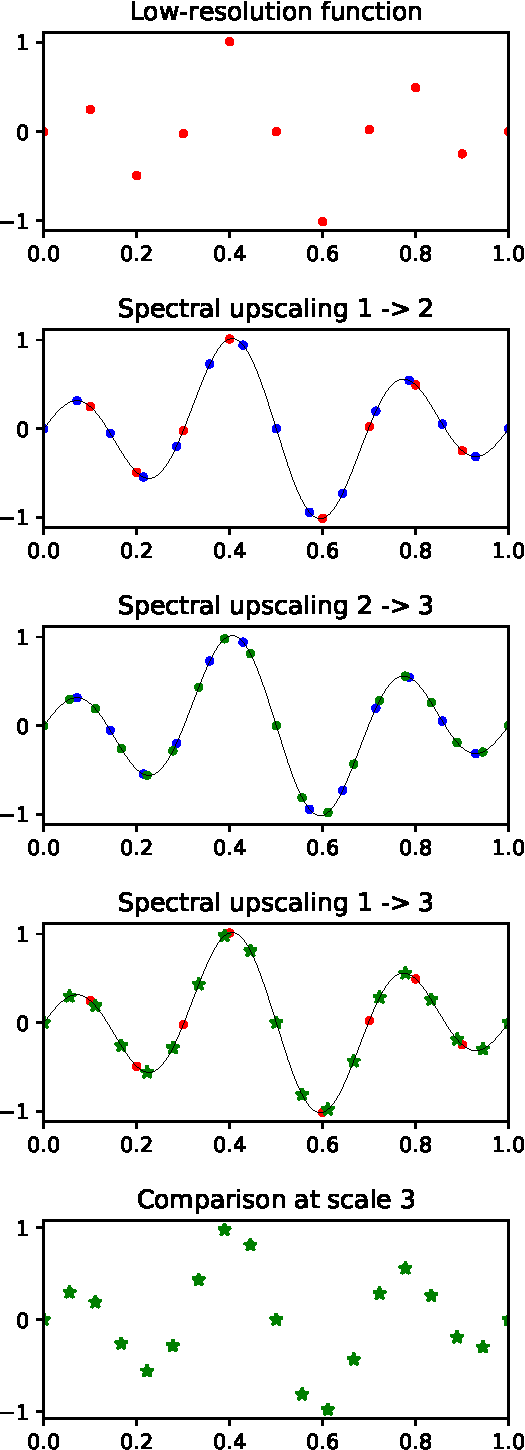
\includegraphics[width=0.45\textwidth]{interpolation_comparison_sp.pdf}
\end{center}
\caption{\label{fig:sp} Transitivity upscaling for a spectral interpolator. Initial low-resolution (red dots), intermediate resolution (blue dots) and high-resolution interpolated from intermediate or low resolution (green dots and stars, respectively). The black lines indicate the continuous interpolation function.}
\end{figure}

\begin{figure}[!h]
\begin{center}
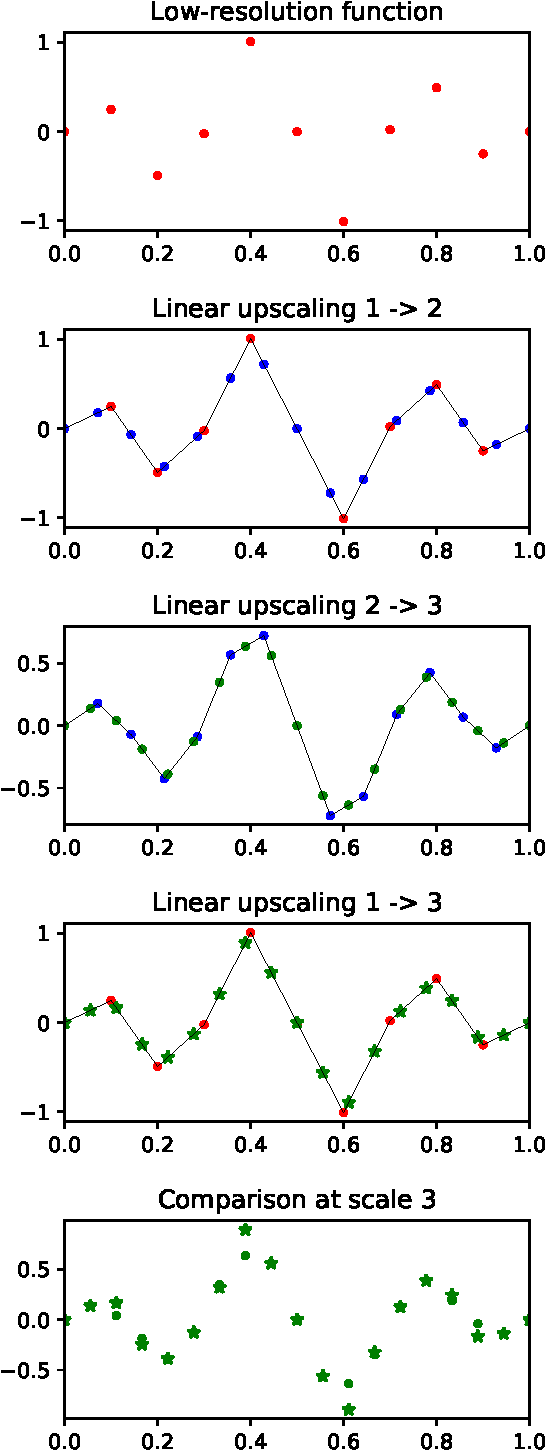
\includegraphics[width=0.45\textwidth]{interpolation_comparison_lin.pdf}
\end{center}
\caption{\label{fig:lin} Transitivity upscaling for a linear interpolator. Initial low-resolution (red dots), intermediate resolution (blue dots) and high-resolution interpolated from intermediate or low resolution (green dots and stars, respectively). The black lines indicate the continuous interpolation functions.}
\end{figure}

\begin{figure}[!h]
\begin{center}
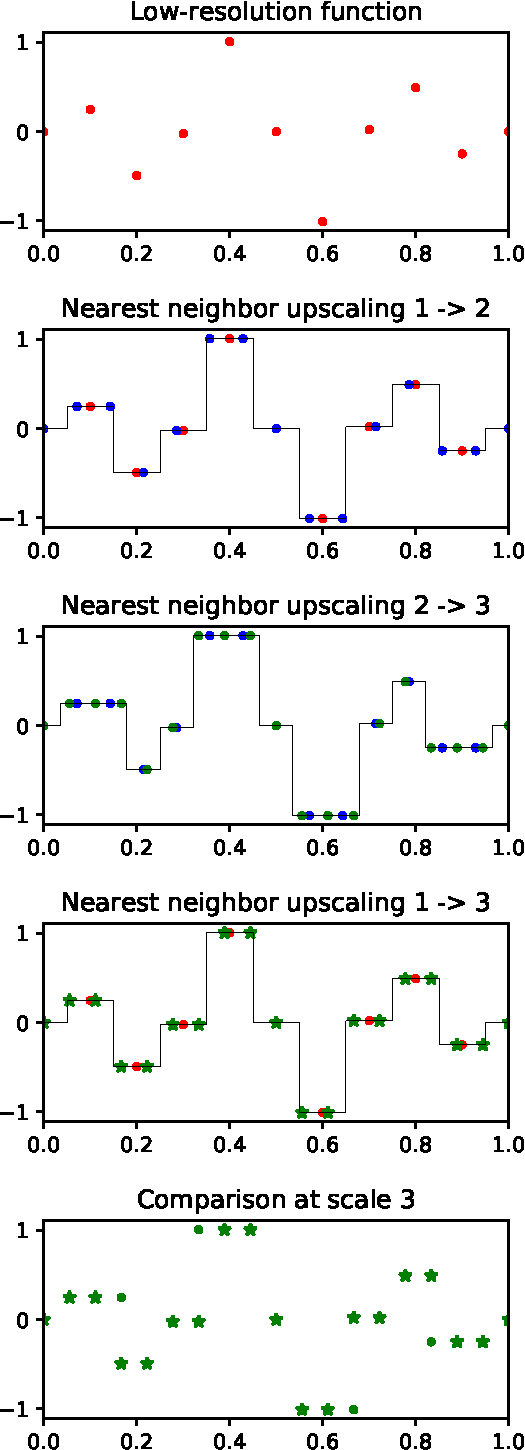
\includegraphics[width=0.45\textwidth]{interpolation_comparison_nn.pdf}
\end{center}
\caption{\label{fig:nn} Transitivity upscaling for a nearest neighbot interpolator. Initial low-resolution (red dots), intermediate resolution (blue dots) and high-resolution interpolated from intermediate or low resolution (green dots and stars, respectively). The black lines indicate the continuous interpolation functions.}
\end{figure}

\subsection{Projective $\mathbf{B}$ family}
The vector $\boldsymbol{\gamma} \in \mathbb{R}^{n_K}$ of positive coefficients is used to define the diagonal matrices $\boldsymbol{\Gamma}_k \in \mathbb{R}^{n_k \times n_k}$:
\begin{align}
\Gamma_{k,\alpha \beta} = \left\{
\begin{array}{ccc}
\gamma_i & \text{ if } & \alpha = \beta \\
0 & \text{ if } & \alpha \ne \beta
\end{array}\right.
\end{align}
At resolution $\mathcal{R}_k$, the background error covariance matrix $\mathbf{B}_k$ is defined as:
\begin{align}
\mathbf{B}_k = \mathbf{S}_k \boldsymbol{\Gamma}_k \mathbf{S}_k^{-1}
\end{align}
Its square-root $\mathbf{U}_k$ is simply:
\begin{align}
\mathbf{U}_k = \mathbf{S}_k \boldsymbol{\Gamma}_k^{1/2} \mathbf{G}_k
\end{align}
where $\mathbf{G}_k \in \mathbb{R}^{n_k \times m_k}$ can be any orthogonal matrix.\\
$  $\\
Thus:
\begin{align}
\mathbf{U}_k^\mathrm{T} \mathbf{T}^\mathbf{x}_{i \rightarrow k} & = \mathbf{G}^\mathrm{T}_k \boldsymbol{\Gamma}_k^{1/2} \mathbf{S}^\mathrm{T}_k \mathbf{S}_k \boldsymbol{\Delta}_{i \rightarrow k} \mathbf{S}^\mathrm{T}_i \nonumber \\
 & = \mathbf{G}^\mathrm{T}_k \boldsymbol{\Gamma}_k^{1/2}\boldsymbol{\Delta}_{i \rightarrow k} \mathbf{S}^\mathrm{T}_i
\end{align}
and
\begin{align}
\mathbf{T}^\mathbf{v}_{i \rightarrow k} \mathbf{U}_i^\mathrm{T} & = \mathbf{G}^\mathrm{T}_k \boldsymbol{\Delta}_{i \rightarrow k} \mathbf{G}_i \mathbf{G}^\mathrm{T}_i \boldsymbol{\Gamma}_i^{1/2} \mathbf{S}^\mathrm{T}_i \nonumber \\
& = \mathbf{G}^\mathrm{T}_k \boldsymbol{\Delta}_{i \rightarrow k}  \boldsymbol{\Gamma}_i^{1/2} \mathbf{S}^\mathrm{T}_i
\end{align}
Since $\boldsymbol{\Gamma}_k^{1/2}\boldsymbol{\Delta}_{i \rightarrow k} = \boldsymbol{\Delta}_{i \rightarrow k}  \boldsymbol{\Gamma}_i^{1/2}$, the projective $\mathbf{B}$ family condition \eqref{eq:projective_definition_U} is verified.

\bibliographystyle{mybib-en}
\bibliography{multi}

\end{document}
